% questions.tex —— 2015 年·四川卷·理科 · 题目内容片段（无答案）
% 由 tools/generate_projects.py 依来源总账自 2015/2015_数学真题_四川理_试题.md 生成，勿手改（改源 MD 后重跑）


\gkpart{数学}

\begin{gktip}
\textbf{来源说明}：本题面依据固定源 PDF 全 2 页逐题核对（p1＝页 981：栏 1 标题与「一、选择题」1–7（含第 3 题框图）；栏 2 第 8–10 题＋「二、填空题」11–15（含第 14 题图）＋「三、解答题」标题（栏尾）；栏 3 第 16、17 题；p2＝页 982：栏 1 第 18、19 题（含双图与四边形图）；栏 2 第 20 题（含椭圆图）；栏 3 第 21 题）。原卷为 \textbf{A3 横向（1190.55 \(\times\) 841.89 pt）三栏书刊合排}，阅读序＝左→中→右；\textbf{页脚仅印合订本书页页码 981／982}（页面底部正中），\textbf{无页眉}。标题「2015 普通高等学校招生考试（四川卷理）」在栏 1 内排印。\textbf{全卷不印分值、不印题量、不印「考生注意」栏}——三处节头逐字仅「一、选择题」「二、填空题」「三、解答题」；总分 150 为结构推断，\textbf{卷面无凭据}，本文件不作补写。

\textbf{源制作体系判定}（\texttt{pdffonts}／\texttt{pdftotext -layout}／\texttt{pdfimages -list} 实测）：源\textbf{不是扫描件，而是 LaTeX（Computer Modern 系）重排产物}——\texttt{pdfimages -list} 零命中（全页无位图；p1 51 条路径＝44 描边＋7 纯填充箭头，p2 39 条＝37 描边＋2 纯填充箭头）；嵌入字体含中文 \textbf{STSong（宋体正文）／STHeiti（黑体标题与节头）}，拉丁与数学 \textbf{LMRoman 系与 CM 系（CMR10／CMMI10／CMSY10／CMEX10／MSAM10／CMR7 等）}，另有 \textbf{TeX-vect10}（专供向量箭头绘制）。文本层整体可读；根号上划线、作答空线、\textbf{「$\parallel$」}（第 18 题 (2)）、全部箭头与向量箭头均为矢量路径。

\textbf{标点与字样约定（实测）}：① \textbf{题号与句末}源内为半角 \texttt{.}（LMRoman10 出字），按全库约定写作全角「．」；② \textbf{正文句读}源内为半角 ASCII（\texttt{, : ; ?}）与半角圆括号，本文件按全库约定归一为全角「，」「：」「；」「？」「（）」，\textbf{顿号「、」与引号「“”」为全角 CJK·照源保留}，内容零改动；③ \textbf{选择题选项标号}源内为\textbf{半角「(A)」照录}；④ \textbf{作答空}：填空题为统一长度横线（实测 31.50 pt，写作 \texttt{\gkblank{}}），选择题作答括注按全库约定写作「（　）」（源为半角括号内留 1 em 空档，实测流内 kern $-$999.952/1000 em）；⑤ \textbf{分数}源内均为显示风格（真分式），排印一律按显示风格（如 \(\dfrac{a}{b}\)）；⑥ \textbf{不等号}按 MSAM10 实测字形排 \(\geqslant\)（字形名 \texttt{greaterorequalslant}，U+2A7E；第 9、21 题）；⑦ \textbf{向量}：本卷源\textbf{无 CMMIB10}——向量字母为 \textbf{CMMI10 常规数学斜体}、箭头为 \textbf{TeX-vect10 伸缩箭头}，一律录作 \(\overrightarrow{AB}\) 类（\textbf{不加粗斜体向量记号}——与同书文卷不同，分卷保留）；⑧ \textbf{常数与函数名}：\(\mathrm{e}\)（第 13 题）、\(\mathrm{i}\)（第 2 题）、\(\lg\)／\(\log\)／\(\sin\)／\(\cos\)／\(\ln\) 源为\textbf{正体}（LMRoman10），照录正体；温度度号源为 CMSY7 的 \(\circ\)，录作 \(^{\circ}\mathrm{C}\)；⑨ \textbf{第 15 题}的两条分式（\(m\)、\(n\) 定义）源为行间尺寸显示式与同行文字共存，本文件按行内显示风格（如 \(\dfrac{a}{b}\)）录入；⑩ \textbf{第 18 题 (2) 的「$\parallel$」}为矢量描边（文本层缺失），按语义排印 \(\parallel\)；⑪ \textbf{词间空格}照页面词界补。

\textbf{存疑与登记}（源内异常一律照录；完整清单见工作档 \texttt{figure-inventory.md} 存疑表 S-1…S-7）：① \textbf{固定源不附参考答案}（等级 D）——本题面无答案区，解析全部由本库独立推导；② \textbf{第 20 题椭圆图动直线与 y 轴交点未精确过 P(0,1)}——按图形自身比例尺（1 单位 = 28.3465 pt = 1 cm）实测交点在 \((0,\ 1.0686)\)（差 1.946 pt），亦非椭圆顶点 \((0,\sqrt{2})\)；图意显系「过 P 的动直线」，\textbf{照源复刻}（直线端点照实测坐标）；③ \textbf{第 18 题右幅直观图非严格斜二测}（前面宽高比 1.06074 $\neq$ 1，系源作图约定）、\textbf{第 14 题图}为 45° 斜投影＋1/2 缩短、\textbf{第 19 题图}按 0.7 cm/单位作图（\(AB/BC/CD/DA\) 与题设 6/3/4/5 逐一对当）；④ \textbf{第 15 题 ③ 须注意 a 充分小时假}（\(a=-2\) 反例）；⑤ 全卷标点为半角拉丁字形，已按全库约定归一全角；⑥ 全卷无分值印制，不录不补。
\end{gktip}

\gkpart{试题}

\gkpart{一、选择题}

\begin{question}
\gkti{1}设集合 \(A=\{x\mid (x+1)(x-2)<0\}\)，集合 \(B=\{x\mid 1<x<3\}\)，则 \(A\cup B=\)（　）

(A) \(\{x\mid -1<x<3\}\)　(B) \(\{x\mid -1<x<1\}\)

(C) \(\{x\mid 1<x<2\}\)　(D) \(\{x\mid 2<x<3\}\)

\end{question}
\begin{question}
\gkti{2}设 \(\mathrm{i}\) 是虚数单位，则复数 \(\mathrm{i}^3-\dfrac{2}{\mathrm{i}}=\)（　）

(A) \(-\mathrm{i}\)　(B) \(-3\mathrm{i}\)　(C) \(\mathrm{i}\)　(D) \(3\mathrm{i}\)

\Needspace{0.4\textheight}
\end{question}
\begin{question}
\gkti{3}执行如图所示的程序框图，输出 \(S\) 的值为（　）
\nopagebreak[4]
\begin{center}% 第 3 题程序框图：按固定源内容流矢量层精确值复刻（1 pt → 0.03515 cm，与全库同制）。
% 原点取框图竖轴 x=216.2232 pt、底缘（结束框底缘）y（顶向下）=509.4991 pt；y 向上（Y = 509.4991 − y_页）。
% 源实测（figure-inventory §1）：
%   7 框 —— 开始/结束＝圆角矩形 27.9988×16.8384 / 27.9988×17.0182（圆角半径 3.9819 横向 × 3.9858 纵向，
%   源为 4 段三次贝塞尔、控制点偏移 2.2000，本图取 rounded corners=0.1400cm 同制）；
%   k=1 矩形 32.0472×14.2905、k=k+1 矩形 50.6793×15.1659、k>4? 菱形 76.0365×18.8821（半对角线 38.0183×9.4410）、
%   S=sin(kπ/6) 矩形 57.2404×28.5967（内嵌真分式故高为数据框的 2 倍强；分数线在源中是独立描边
%   x 227.9894–240.1463 @ y=433.1499，本图由 \dfrac 自带分数线渲染）、
%   输出 S 平行四边形 50.8121×16.8579（斜边水平偏移 6.1351，上边偏右）。
%   连线 6 条竖直（竖轴 x=0，箭尖照源实测；源三角 2.9855 宽 × 3.9820 高，尖端向下）；
%   「否」支 3 段回折 —— 自菱形右顶点右行 (38.2997→52.4730)、竖直上行 (115.7156→162.2645)、
%   水平左行至竖轴 x=0，箭尖 (0,162.2645) 恰落在 k=1 框底与 k=k+1 框顶的正中点（源实测落点
%   y_页=347.2346 与两框间隙中点 347.2327 差 0.0019）——即回流到 k=k+1 的入线正中，
%   判定为当型循环；实心箭头共 7 枚（6 下 + 1 左）。全图无虚线、无圆形节点。
%   以下坐标均为本图坐标系（X = x_页 − 216.2232，Y = 509.4991 − y_页），与代码逐值一致。
%   框内文字与分支标签一律按源字形盒并集中心定位（figure-inventory §1.4）。
\begin{tikzpicture}[x=0.03515cm,y=0.03515cm,>=stealth,every node/.style={font=\small,inner sep=0pt}]
% ===== 7 框（外轮廓照源实测值）=====
\draw[line width=0.398bp,rounded corners=0.1400cm] (-13.9974,198.4148) rectangle (14.0014,215.2532); % 1 开始（圆角）
\draw[line width=0.398bp] (-16.0216,169.5524) rectangle (16.0256,183.8429);                            % 2 k=1
\draw[line width=0.398bp] (-25.3377,139.8146) rectangle (25.3416,154.9805);                            % 3 k=k+1
\draw[line width=0.398bp] (0,125.1567)--(38.0183,115.7156)--(0,106.2746)--(-38.0182,115.7156)--cycle;  % 4 菱形 k>4?
\draw[line width=0.398bp] (-28.6202,63.0200) rectangle (28.6202,91.6167);                              % 5 S=sin(kπ/6)
\draw[line width=0.398bp] (-25.4080,31.5901)--(-19.2729,48.4480)--(25.4041,48.4480)--(19.2690,31.5901)--cycle; % 6 输出 S
\draw[line width=0.398bp,rounded corners=0.1400cm] (-13.9974,0) rectangle (14.0014,17.0182);            % 7 结束（圆角）
% ===== 连线（6 竖直 + 1 回折；箭尖照源实测）=====
\draw[->,line width=0.398bp] (0,198.2155)--(0,184.0422);   % 开始→k=1
\draw[->,line width=0.398bp] (0,169.3531)--(0,155.1798);   % k=1→k=k+1（回折靶线）
\draw[->,line width=0.398bp] (0,139.6153)--(0,125.4420);   % k=k+1→菱形顶
\draw[->,line width=0.398bp] (0,105.9932)--(0,91.8199);    % 菱形底→S=sin（是支）
\draw[->,line width=0.398bp] (0,62.8245)--(0,48.6512);     % S=sin→输出 S
\draw[->,line width=0.398bp] (0,31.3908)--(0,17.2175);     % 输出 S→结束
\draw[->,line width=0.398bp] (38.2997,115.7156)--(52.4730,115.7156)--(52.4730,162.2645)--(0,162.2645); % 否支回折（回流 k=k+1 入线正中）
% ===== 框内文字与分支标签（照源字形盒并集中心定位）=====
\node at (-0.0002,207.4161) {开始};
\node at (-0.0047,175.6761) {\(k=1\)};
\node at (-0.0017,146.8131) {\(k=k+1\)};
\node at (-0.0007,114.8451) {\(k>4?\)};
\node at (-0.5981,76.3001) {\(S=\sin\dfrac{k\pi}{6}\)};
\node at (-0.3052,40.3496) {输出 \(S\)};
\node at (-0.0002,9.1181) {结束};
\node at (-8.9492,99.5931) {是};
\node at (38.2988,124.6861) {否};
\end{tikzpicture}
\end{center}
\nopagebreak[4]
(A) \(-\dfrac{\sqrt{3}}{2}\)　(B) \(\dfrac{\sqrt{3}}{2}\)　(C) \(-\dfrac{1}{2}\)　(D) \(\dfrac{1}{2}\)

\end{question}
\begin{question}
\gkti{4}下列函数中，最小正周期为 \(\pi\) 且图象关于原点对称的函数是（　）

(A) \(y=\cos\left(2x+\dfrac{\pi}{2}\right)\)　(B) \(y=\sin\left(2x+\dfrac{\pi}{2}\right)\)

(C) \(y=\sin 2x+\cos 2x\)　(D) \(y=\sin x+\cos x\)

\end{question}
\begin{question}
\gkti{5}过双曲线 \(x^2-\dfrac{y^2}{3}=1\) 的右焦点且与 \(x\) 轴垂直的直线，交该双曲线的两条渐近线于 \(A\)，\(B\) 两点，\(|AB| =\)（　）

(A) \(\dfrac{4\sqrt{3}}{3}\)　(B) \(2\sqrt{3}\)　(C) \(6\)　(D) \(4\sqrt{3}\)

\end{question}
\begin{question}
\gkti{6}用数字 0，1，2，3，4，5 组成没有重复数字的五位数，其中比 40000 大的偶数共有（　）

(A) 144 个　(B) 120 个　(C) 96 个　(D) 72 个

\end{question}
\begin{question}
\gkti{7}设四边形 \(ABCD\) 为平行四边形，\(\left|\overrightarrow{AB}\right|=6\)，\(\left|\overrightarrow{AD}\right|=4\)．若点 \(M\)，\(N\) 满足 \(\overrightarrow{BM}=3\overrightarrow{MC}\)，\(\overrightarrow{DN}=2\overrightarrow{NC}\)，则 \(\overrightarrow{AM}\cdot\overrightarrow{NM}=\)（　）

(A) 20　(B) 15　(C) 9　(D) 6

\end{question}
\begin{question}
\gkti{8}设 \(a\)，\(b\) 都是不等于 1 的正数，则“\(3^a>3^b>3\)”是“\(\log_a 3<\log_b 3\)”的（　）

(A) 充要条件　(B) 充分不必要条件

(C) 必要不充分条件　(D) 既不充分也不必要条件

\end{question}
\begin{question}
\gkti{9}如果函数 \(f(x)=\dfrac{1}{2}(m-2)x^2+(n-8)x+1\)（\(m\geqslant 0\)，\(n\geqslant 0\)）在区间 \(\left[\dfrac{1}{2},2\right]\) 上单调递减，那么 \(mn\) 的最大值为（　）

(A) 16　(B) 18　(C) 25　(D) \(\dfrac{81}{2}\)

\end{question}
\begin{question}
\gkti{10}设直线 \(l\) 与抛物线 \(y^2=4x\) 相交于 \(A\)，\(B\) 两点，与圆 \((x-5)^2+y^2=r^2\)（\(r>0\)）相切于点 \(M\)，且 \(M\) 为线段 \(AB\) 的中点．若这样的直线 \(l\) 恰有 4 条，则 \(r\) 的取值范围是（　）

(A) \((1,3)\)　(B) \((1,4)\)　(C) \((2,3)\)　(D) \((2,4)\)

\end{question}
\gkpart{二、填空题}

\begin{question}
\gkti{11}在 \((2x-1)^5\) 的展开式中，含 \(x^2\) 的项的系数是\gkblank{}．（用数字填写答案）

\end{question}
\begin{question}
\gkti{12}\(\sin 15^{\circ}+\sin 75^{\circ}\) 的值是\gkblank{}．

\end{question}
\begin{question}
\gkti{13}某食品的保鲜时间 \(y\)（单位：小时）与储藏温度 \(x\)（单位：\(^{\circ}\mathrm{C}\)）满足函数关系 \(y=\mathrm{e}^{kx+b}\)（\(\mathrm{e}=2.718\cdots\) 为自然对数的底数，\(k\)，\(b\) 为常数）．若该食品在 \(0^{\circ}\mathrm{C}\) 的保鲜时间是 192 小时，在 \(22^{\circ}\mathrm{C}\) 的保鲜时间是 48 小时，则该食品在 \(33^{\circ}\mathrm{C}\) 的保鲜时间是\gkblank{}小时．

\Needspace{0.4\textheight}
\end{question}
\begin{question}
\gkti{14}如图，四边形 \(ABCD\) 和 \(ADPQ\) 均为正方形，它们所在的平面互相垂直，动点 \(M\) 在线段 \(PQ\) 上，\(E\)，\(F\) 分别为 \(AB\)，\(BC\) 的中点．设异面直线 \(EM\) 与 \(AF\) 所成的角为 \(\theta\)，则 \(\cos\theta\) 的最大值为\gkblank{}．
\nopagebreak[4]
\begin{center}% 第 14 题图（四边形 ABCD ＋ 正方形 ADPQ，面面垂直示意）：按固定源内容流矢量层精确值复刻（1 pt → 0.03515 cm，与全库同制）。
% 原点取 A 的 x=527.1415 pt、底缘（F 标签下缘）y（顶向下）=636.8870 pt；y 向上（Y = 636.8870 − y_页）。
% 源实测（figure-inventory §2）：3 条路径、9 条直线段，全实线、无虚线、无填充、无箭头，线宽 0.398。
%   正方形 ADPQ 按真形画出（轴对齐矩形，AD=102.0503、AQ=102.0463，差 0.0040 ⇒ 正方形）；
%   四边形 ABCD 按 45° 斜投影 + 1/2 缩短画成平行四边形（AB=51.0166 @ 44.997°、BC=102.0464、
%   CD=51.0138、DA=102.0503 —— AB/AD=0.49992≈1/2，与题干「ABCD 为正方形」自洽，属源内作图约定 S-2）。
%   E 为 AB 中点（源 p45 起点页 pt (545.1796,606.2505)，与中点解析值差 0.0019，本图照 p45 起点抄录）、
%   F 为 BC 中点（与 p44 末段终点逐位一致）、M 在 PQ 上、按源选定位置画在 Q→P 的 3/4 处
%   （归一化 0.749990 —— M 是动点，源取的代表位置非中点，照源保留，见 S-6）。
%   线段 9 条＝四边形 4（AB、BC、CD、DA，DA 为两面的公共棱）+ 正方形 3（DP、PQ、QA）+ AF + EM；
%   图中不画对角线，也无 EB/BF 之外的辅助线。标签 9 个（A、B、C、D、E、F、M、P、Q），照源字形盒中心定位。
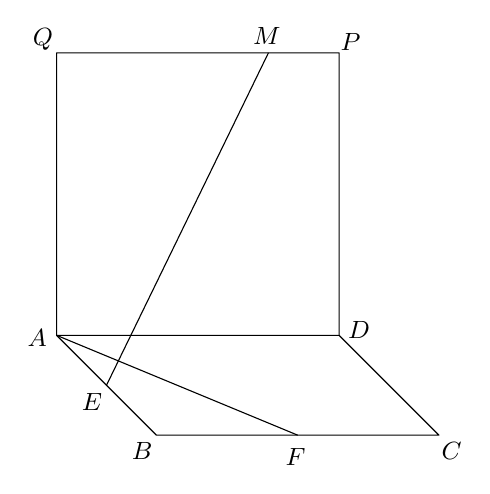
\begin{tikzpicture}[x=0.03515cm,y=0.03515cm,every node/.style={font=\small,inner sep=0pt},
  gl/.style={line width=0.398bp,line join=round}]
% ===== p43：四边形 ABCD（AB–BC–CD–DA；DA 为四边形与正方形的公共棱）=====
\draw[gl] (0,48.6707)--(36.0761,12.5985)--(138.1225,12.5985)--(102.0503,48.6707)--cycle;
% ===== p44：正方形 ADPQ（DP–PQ–QA）＋ 线段 AF（F 为 BC 中点）=====
\draw[gl] (102.0503,48.6707)--(102.0503,150.7170)--(0,150.7170)--(0,48.6707)--(87.0993,12.5985);
% ===== p45：线段 EM（E 为 AB 中点，M 在 PQ 的 Q→P 3/4 处）=====
\draw[gl] (18.0381,30.6365)--(76.5367,150.7170);
% ===== 标签 9 个（照源字形盒中心定位）=====
\node at (-4.9310,155.7090) {\(Q\)};
\node at (75.9635,156.7310) {\(M\)};
\node at (106.2500,154.6880) {\(P\)};
\node at (109.2650,50.7590) {\(D\)};
\node at (-6.9730,47.7090) {\(A\)};
\node at (12.8030,24.7410) {\(E\)};
\node at (30.8795,6.7040) {\(B\)};
\node at (86.3690,4.6620) {\(F\)};
\node at (142.6775,6.7040) {\(C\)};
\end{tikzpicture}
\end{center}
\nopagebreak[4]
\end{question}
\begin{question}
\gkti{15}已知函数 \(f(x)=2^x\)，\(g(x)=x^2+ax\)（其中 \(a\in\mathbf{R}\)）．对于不相等的实数 \(x_1\)，\(x_2\)，设 \(m=\dfrac{f(x_1)-f(x_2)}{x_1-x_2}\)，\(n=\dfrac{g(x_1)-g(x_2)}{x_1-x_2}\)，现有如下命题：

① 对于任意不相等的实数 \(x_1\)，\(x_2\)，都有 \(m>0\)；

② 对于任意的 \(a\) 及任意不相等的实数 \(x_1\)，\(x_2\)，都有 \(n>0\)；

③ 对于任意的 \(a\)，存在不相等的实数 \(x_1\)，\(x_2\)，使得 \(m=n\)；

④ 对于任意的 \(a\)，存在不相等的实数 \(x_1\)，\(x_2\)，使得 \(m=-n\)．

其中的真命题有\gkblank{}．（写出所有真命题的序号）

\end{question}
\gkpart{三、解答题}

\begin{question}
\gkti{16}设数列 \(\{a_n\}\)（\(n=1,2,3,\cdots\)）的前 \(n\) 项和 \(S_n\) 满足 \(S_n=2a_n-a_1\)，且 \(a_1\)，\(a_2+1\)，\(a_3\) 成等差数列．

（1） 求数列 \(\{a_n\}\) 的通项公式；

（2） 记数列 \(\left\{\dfrac{1}{a_n}\right\}\) 的前 \(n\) 项和为 \(T_n\)，求使得 \(|T_n-1|<\dfrac{1}{1000}\) 成立的 \(n\) 的最小值．

\end{question}
\begin{question}
\gkti{17}某市 \(A\)，\(B\) 两所中学的学生组队参加辩论赛，\(A\) 中学推荐了 3 名男生、2 名女生，\(B\) 中学推荐了 3 名男生、4 名女生，两校所推荐的学生一起参加集训．由于集训后队员水平相当，从参加集训的男生中随机抽取 3 人、女生中随机抽取 3 人组成代表队．

（1） 求 \(A\) 中学至少有 1 名学生入选代表队的概率；

（2） 某场比赛前，从代表队的 6 名队员中随机抽取 4 人参赛，设 \(X\) 表示参赛的男生人数，求 \(X\) 的分布列和数学期望．

\Needspace{0.4\textheight}
\end{question}
\begin{question}
\gkti{18}一个正方体的平面展开图及该正方体的直观图的示意图如图所示．在正方体中，设 \(BC\) 的中点为 \(M\)，\(GH\) 的中点为 \(N\)．
\nopagebreak[4]
\begin{center}% 第 18 题正方体平面展开图＋直观图（两幅一体）：按固定源内容流矢量层精确值复刻（1 pt → 0.03515 cm，与全库同制）。
% 原点取展开图左缘（横条外轮廓左边）x=174.1018 pt、底缘（直观图 A/B 标签下缘）y（顶向下）=267.1130 pt；y 向上（Y = 267.1130 − y_页）。
% 源实测（figure-inventory §3）：
% 左幅（展开图）：十字六连方（竖条 1×4 叠横条 3×1，共用中格 M）；格边长 28.3466＝1.0000 cm，每格严格正方形；
%   竖条轮廓 x 28.3467–56.6933、y 12.9096–126.3001；横条轮廓 x 0–85.0400、y 69.6068–97.9534；
%   竖条内部第 3 条格线 @ y 41.2602（R3/R4 分界）。8 个字母全部贴网格顶点排印、无一落在格内（§3.1.1）。
% 右幅（直观图）：8 顶点 / 12 棱（9 实 + 3 虚；虚线节距 2.98883，三条均自隐藏顶点 BBL 出发）；
%   前面 68.0374 × 64.1414（宽高比 1.06074 ≠ 1 —— 不是严格斜二测，深度方向却严格 44.995°、
%   长 34.0120 ≈ 前面宽之半；属源内作图约定，照源复刻不改画，见 §7.2 S-1）；
%   M 为 BC 中点（源页 pt (377.7569,244.5318)＝本图 (203.6551,22.5812)），图上另画实心圆点
%   （全图唯一圆点，直径 2.4 pt），字母 M 排于圆点右下。
% 注：除注明「源页 pt」者外，本注释内坐标均为本图坐标系（X = x_页 − 174.1018，Y = 267.1130 − y_页）。
\begin{tikzpicture}[x=0.03515cm,y=0.03515cm,every node/.style={font=\small,inner sep=0pt},
  gl/.style={line width=0.3985bp,line join=round}]
% ===== 左幅：平面展开图（十字六连方，格边长 28.3466）=====
\draw[gl] (28.3467,12.9096) rectangle (56.6933,126.3001);   % 竖条外轮廓（1×4）
\draw[gl] (0,69.6068) rectangle (85.0400,97.9534);          % 横条外轮廓（3×1）
\draw[gl] (28.3467,41.2602)--(56.6933,41.2602);             % 竖条内部第 3 条格线（R3/R4 分界）
% ===== 左幅字母（照源字形盒中心定位；全部锚于格点、不在格内）=====
\node at (20.0097,104.2760) {\(D\)};
\node at (64.1452,104.2760) {\(C\)};
\node at (92.8677,104.2760) {\(G\)};
\node at (-8.1793,61.3570) {\(E\)};
\node at (20.7107,61.3570) {\(A\)};
\node at (64.3752,61.3570) {\(B\)};
\node at (63.7697,40.2960) {\(F\)};
\node at (19.4317,4.6630) {\(H\)};
% ===== 右幅：正方体直观图（顶点照源实测）=====
% 实线 9 条
\draw[gl] (123.5936,10.5572)--(191.6310,10.5572);   % 前面下边（A–B）
\draw[gl] (191.6310,10.5572)--(215.6792,34.6053);   % 右面下边（B–C）
\draw[gl] (123.5936,74.6986)--(191.6310,74.6986);   % 前面上边
\draw[gl] (191.6310,74.6986)--(215.6792,98.7506);   % 右面上边
\draw[gl] (215.6792,98.7506)--(147.6457,98.7506);   % 顶面后边
\draw[gl] (147.6457,98.7506)--(123.5936,74.6986);   % 顶面左边
\draw[gl] (191.6310,74.6986)--(191.6310,10.5572);   % 前/右公共竖棱
\draw[gl] (215.6792,98.7506)--(215.6792,34.6053);   % 后面右边
\draw[gl] (123.5936,74.6986)--(123.5936,10.5572);   % 前面左边
% 虚线 3 条（照源节距 2.98883；均自隐藏顶点 BBL=(147.6457,34.6053) 出发）
\draw[gl,dash pattern=on 2.98883pt off 2.98883pt] (123.5936,10.5572)--(147.6457,34.6053);  % 底面左边（A→隐藏点）
\draw[gl,dash pattern=on 2.98883pt off 2.98883pt] (147.6457,34.6053)--(215.6792,34.6053);  % 底面后边
\draw[gl,dash pattern=on 2.98883pt off 2.98883pt] (147.6457,34.6053)--(147.6457,98.7506);  % 后面左边
% ===== 右幅：BC 中点 M 处的实心圆点（源为字形 • ，中心与 BC 中点逐位吻合）=====
\fill (203.6551,22.5812) circle [radius=1.2000];
% ===== 右幅字母（照源字形盒中心定位）=====
\node at (118.3597,78.6700) {\(E\)};
\node at (140.1347,36.6940) {\(D\)};
\node at (222.2782,33.6440) {\(C\)};
\node at (118.6617,4.6620) {\(A\)};
\node at (196.2972,4.6620) {\(B\)};
\node at (208.0132,16.6880) {\(M\)};
\end{tikzpicture}
\end{center}
\nopagebreak[4]
（1） 请将字母 \(F\)，\(G\)，\(H\) 标记在正方体相应的顶点处（不需说明理由）；

（2） 证明：直线 \(MN\parallel\) 平面 \(BDH\)；

（3） 求二面角 \(A-EG-M\) 的余弦值．

\Needspace{0.4\textheight}
\end{question}
\begin{question}
\gkti{19}如图，\(A\)，\(B\)，\(C\)，\(D\) 为平面四边形 \(ABCD\) 的四个内角．
\nopagebreak[4]
\begin{center}% 第 19 题四边形图：按固定源内容流矢量层精确值复刻（1 pt → 0.03515 cm，与全库同制）。
% 原点取 A 的 x=272.6508 pt、底缘（A/B 标签下缘）y（顶向下）=630.2490 pt；y 向上（Y = 630.2490 − y_页）。
% 源实测（figure-inventory §4）：4 条边＝4 条独立路径（全实线、无填充、无箭头、线宽 0.3985；对角线不画）。
%   顶点 A(272.6508,619.6931)、B(391.7075,619.6931)、C(388.5344,560.1628)、D(315.1121,530.0029)；
%   AB 严格水平（两端 y 逐位相同）；BC 接近竖直（Δx=−3.1731）。
%   实长 DA=99.2335 / DC=79.3754 / BA=119.0567 / BC=59.6148，折 cm 为 3.5007/2.8002/4.2000/2.1031，
%   以 0.7 cm 为单位即 5.0010/4.0003/6.0001/3.0044 ≈ 5/4/6/3，与题干 AB=6、BC=3、CD=4、AD=5
%   逐一对应（偏差 ≤0.0015 单位）⇒ 本图按 0.7 cm/单位按比例作图、角度亦按真值，重绘须保留（S-3）。
\begin{tikzpicture}[x=0.03515cm,y=0.03515cm,every node/.style={font=\small,inner sep=0pt},
  gl/.style={line width=0.3985bp,line join=round}]
% ===== 四条边（各为独立路径，照源写法）=====
\draw[gl] (42.4613,100.2461)--(0,10.5559);          % DA
\draw[gl] (42.4613,100.2461)--(115.8836,70.0862);   % DC
\draw[gl] (119.0567,10.5559)--(0,10.5559);          % BA
\draw[gl] (119.0567,10.5559)--(115.8836,70.0862);   % BC
% ===== 标签 4 个（照源字形盒中心定位）=====
\node at (-4.9333,4.6620) {\(A\)};
\node at (123.7242,4.6620) {\(B\)};
\node at (120.4372,74.0540) {\(C\)};
\node at (42.3167,108.2510) {\(D\)};
\end{tikzpicture}
\end{center}
\nopagebreak[4]
（1） 证明：\(\tan\dfrac{A}{2}=\dfrac{1-\cos A}{\sin A}\)；

（2） 若 \(A+C=180^{\circ}\)，\(AB=6\)，\(BC=3\)，\(CD=4\)，\(AD=5\)，求 \(\tan\dfrac{A}{2}+\tan\dfrac{B}{2}+\tan\dfrac{C}{2}+\tan\dfrac{D}{2}\) 的值．

\Needspace{0.4\textheight}
\end{question}
\begin{question}
\gkti{20}如图，椭圆 \(E:\dfrac{x^2}{a^2}+\dfrac{y^2}{b^2}=1\)（\(a>b>0\)）的离心率是 \(\dfrac{\sqrt{2}}{2}\)，过点 \(P(0,1)\) 的动直线 \(l\) 与椭圆相交于 \(A\)，\(B\) 两点．当直线 \(l\) 平行于 \(x\) 轴时，直线 \(l\) 被椭圆 \(E\) 截得的线段长为 \(2\sqrt{2}\)．
\nopagebreak[4]
\begin{center}% 第 20 题椭圆图：按固定源内容流矢量层精确值复刻（1 pt → 0.03515 cm，与全库同制）。
% 原点取 x 轴负端 x=616.6363 pt、y 轴下端 y（顶向下）=301.4517 pt；y 向上（Y = 301.4517 − y_页）。
% 源实测（figure-inventory §5）：中心 O=(76.5367,56.6933)、半轴 a=56.6933 / b=40.0815，a/b=1.414451≈√2；
%   椭圆线宽 0.79701bp（其余线的 2 倍，全卷唯一加粗线——突出二次曲线，照源）；x 轴、y 轴、割线线宽 0.3985；
%   4 段三次贝塞尔闭合，控制点偏移比 0.55225(x)/0.55231(y)≈0.55228，本图用 TikZ ellipse 同制。
%   作图比例尺 1 cm = 1 单位（a=2.00000 cm、b=1.41435 cm），椭圆即 x²/4+y²/2=1（题干 (1) 的答案）。
%   x 轴自左端过中心向右，线段末端 149.4861、箭尖 153.0734（至左端左右对称外伸 19.8434）；
%   y 轴自下端过中心向上，线段上端 112.6324、箭尖 116.2197（上端外伸 19.4449）；两箭头为源内纯填充三角（2.9894×3.9859）。
%   全图 3 直线段 + 1 椭圆 + 2 枚箭头，无虚线、无区域填充、无点标记；标签 6 个（x、y、A、B、P、O），
%   照源字形盒中心定位；图上不标椭圆顶点与焦点。
% 源内异常（照源复刻、已登记，见 §5.3 E-1）：割线 l 实测端点 (13.4933,37.7056)–(104.3128,108.6973)、
%   长 115.2899、斜率 −0.781676，与 y 轴交点 y=1.0686 单位 ≠ 题干 P(0,1) 的 1.0000（差 1.946 pt），
%   且为两端伸出椭圆外的延长割线。**此处照源实测端点抄录，勿按题干「修正」为过 (0,1)**。
% 注：本注释内坐标均为本图坐标系（X = x_页 − 616.6363，Y = 301.4517 − y_页），与代码逐值一致。
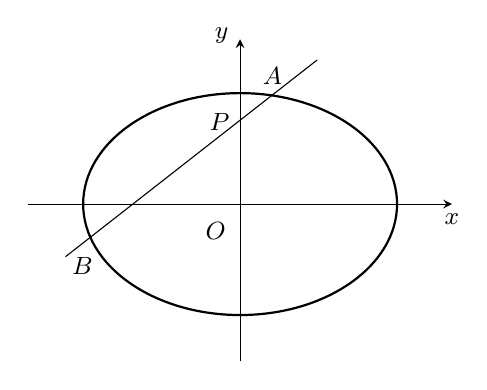
\begin{tikzpicture}[x=0.03515cm,y=0.03515cm,>=stealth,every node/.style={font=\small,inner sep=0pt}]
% ===== 椭圆（4 段贝塞尔，线宽 0.79701 为全卷唯一加粗）=====
\draw[line width=0.79701bp] (76.5367,56.6933) ellipse [x radius=56.6933, y radius=40.0815];
% ===== 两轴与箭头（照源：直线段 + 独立填充三角，此处并入线端）=====
\draw[line width=0.3985bp] (0,56.6933)--(149.4861,56.6933);           % x 轴（线段，右端）
\draw[->,line width=0.3985bp] (149.4861,56.6933)--(153.0734,56.6933); % x 轴箭头（尖端照源）
\draw[line width=0.3985bp] (76.5367,0)--(76.5367,112.6324);           % y 轴（线段，上端）
\draw[->,line width=0.3985bp] (76.5367,112.6324)--(76.5367,116.2197); % y 轴箭头（尖端照源）
% ===== 割线 l（过 P 的动直线；照源实测端点，两端伸出椭圆外）=====
\draw[line width=0.3985bp] (13.4933,37.7056)--(104.3128,108.6973);
% ===== 标签 6 个（照源字形盒中心定位）=====
\node at (69.8847,117.6067) {\(y\)};
\node at (88.2192,103.1367) {\(A\)};
\node at (69.0962,86.1807) {\(P\)};
\node at (67.6922,47.0137) {\(O\)};
\node at (19.5517,34.4447) {\(B\)};
\node at (153.0712,51.0977) {\(x\)};
\end{tikzpicture}
\end{center}
\nopagebreak[4]
（1） 求椭圆 \(E\) 的方程；

（2） 在平面直角坐标系 \(xOy\) 中，是否存在与点 \(P\) 不同的定点 \(Q\)，使得 \(\dfrac{|QA|}{|QB|}=\dfrac{|PA|}{|PB|}\) 恒成立？若存在，求出点 \(Q\) 的坐标；若不存在，请说明理由．

\end{question}
\begin{question}
\gkti{21}已知函数 \(f(x)=-2(x+a)\ln x+x^2-2ax-2a^2+a\)，其中 \(a>0\)．

（1） 设 \(g(x)\) 是 \(f(x)\) 的导函数，讨论 \(g(x)\) 的单调性；

（2） 证明：存在 \(a\in(0,1)\)，使得 \(f(x)\geqslant 0\) 在区间 \((1,+\infty)\) 内恒成立，且 \(f(x)=0\) 在区间 \((1,+\infty)\) 内有唯一解．

\end{question}